\documentclass{article}
\usepackage{tikz}
\setlength{\parindent}{0mm}
\usetikzlibrary{intersections,calc}
\begin{document}
% 坐标点类型
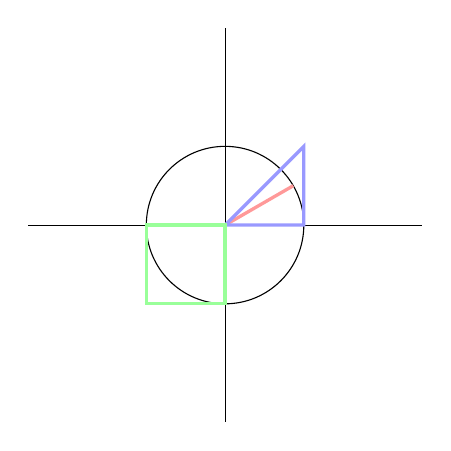
\begin{tikzpicture}
    % (-2.5,0)为普通点坐标
    \draw (-2.5,0) -- (2.5,0);
    \draw (0,-2.5) -- (0,2.5);
    \draw (0,0) circle [radius=1];
    
    % (30:1)为基于圆的极坐标,30代表逆时针30度,1代表2cm的圆半径长度
    % 可以使用基于椭圆的极坐标(30:1cm and 2cm)
    \draw[red!40,very thick] (0,0) -- (30:1);
    
    % +(0,1)为相对于当前坐标点的坐标,但不更新到当前坐标点
    \draw[blue!40,very thick] (0,0) -- (1,0) -- +(0,1) -- +(-1,0); 

    % ++(0,-1)为相对于当前坐标点的坐标,并且更新到当前坐标点
    \draw[green!40,very thick] (0,0) -- (-1,0) -- ++(0,-1) -- ++(1,0) -- cycle; 
\end{tikzpicture}\\\vspace{1cm}

\begin{tikzpicture}
    % 命名坐标点
    \coordinate (A) at (-1,-1);
    \coordinate (B) at (-1,1);
    \coordinate (C) at (1,1);
    \coordinate (D) at (1,-1);
    \draw[->] (-2,0) -- (2,0) node[right] {$x$};
    \draw[->] (0,-2) -- (0,2) node[above] {$y$};
    \draw (A) -- (B) -- (C) -- (D) -- cycle;
\end{tikzpicture}\\\vspace{1cm}

\begin{tikzpicture}
    % 复杂计算
    \draw (0,0) circle [radius=2];
    % \pgfmathparse{<complex_calculate>}
    %   复杂计算(包含函数等),结果不包含单位
    %   其他简单计算会全部转化为pt单位
    % \pgfmathresult
    %   将上一次\pgfmathparse计算结果进行引用
    \filldraw (1,\pgfmathparse{sqrt(3)}\pgfmathresult) circle [radius=2pt];
    \draw (0,0) circle [radius=3];
    \fill[green] (1,\pgfmathparse{2*sqrt(2)}\pgfmathresult) circle [radius=2pt];
    
    % 常用函数
    % sqrt(<num>)
    %   求平方根
    % sin(<degree>)
    %   求正弦值
    %   参数为角度格式,可使用<radian> r将弧度转化为角度
    % asin(<val>)
    %   求反正弦值, 值域[-90,90]
    %   返回值为角度值  
    % atan(<val>)
    %    求反正切值
    % atan2(y,x)
    %    求y/x的反正切值
\end{tikzpicture}\vspace{1cm}

\begin{tikzpicture}
    % p |- q,取p坐标的x值,取q坐标的y值
    % p -| q,取p坐标的y值,取q坐标的x值
    \draw (-2.5,0) -- (2.5,0) coordinate(x axis);
    \draw (0,-2.5) -- (0,2.5);
    \draw (0,0) circle [radius=2];
    \fill[red] (30:2 |- x axis) circle [radius=2pt];
    \draw[blue] (30:2) -- (30:2 |- x axis);
\end{tikzpicture}\\\vspace{1cm}

\begin{tikzpicture}
    % 直接对坐标点进行移动_1
    \coordinate (A) at (0,0);
    \coordinate (B) at (3,0);
    \coordinate (C) at ([shift=(B)]A);
    \coordinate (D) at ([shift={(3,0)}]A);
    \draw (A) -- (C);
\end{tikzpicture}\\\vspace{1cm}

\begin{tikzpicture}
    % 直接对坐标点进行移动_2
    \draw[-stealth] (-2,0) -- (2,0) node[pos=1,below]{$x$};
    \draw[-stealth] (0,-2) -- (0,2) node[pos=1,right]{$y$};
    \foreach \x in {-1.5,-1,-0.5,0.5,1,1.5}
        \draw (\x,0) -- (\x,2pt);
    \foreach \y in {-1.5,-1,-0.5,0.5,1,1.5}
        \draw (0,\y) -- (2pt,\y);
    \filldraw (0,0) circle [radius=1.2pt];
    \filldraw ([rotate around={-90:(0.5,0)}]1,0) circle [radius=1.2pt];
\end{tikzpicture}

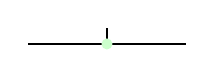
\begin{tikzpicture}
    % 在指定线段上取一个点. 需要使用calc库
    % 格式1: <point_start>!<percent>!<point_end>
    % 沿着point_start到point_end直线,指定百分比位置,percent可以小于0,也可以大于1
    % 格式2: <point_start>!<percent>!<angle>:<point_end>
    % 绕起始点point_start旋转指定角度angle,然后从结果线段上截取指定百分比位置
    % 格式3: <point_start>!<length>!<point_end>
    % 沿着point_start到point_end直线,距离起始点point_start长度为length的位置
    % 格式4: <point_start>!<length>!<angle>:<point_end>
    % 绕起始点point_start旋转指定角度angle,然后从结果线段上截取距离起始点长度为length的位置
    % 格式5: <point_start>!<point>!<point_end>
    % 由点<point>,到由<point_start>和<point_end>组成的线段的垂足
    % 格式6: <point_start>!<point>!<angle>:<point_end>
    % 由<point_start>和<point_end>组成的线段,旋转指定角度angle后,过点point到该线段的垂足

    \coordinate (A) at (0,0);
    \coordinate (B) at (2,0);
    \coordinate (C) at ($ (A)!0.5!(B) $);

    \draw (A) -- (B);
    \draw (1,0) -- (1,0.2);
    \fill[green!20] (C) circle [radius=2pt];
\end{tikzpicture}\\\vspace{1cm}

% 路径
\begin{tikzpicture}
    % 直线与直线的交点,需要使用intersections库
    \path [draw,name path=x axis](-2,0) -- (2,0);
    \path [draw,name path=y axis](0,-2) -- (0,2);

    % of参数,相交的两条路径, 格式为<path_01> and <path_02>
    % by参数,相交点的坐标,可使用{}限定多个相交点
    % name参数,相交点的名称,用于后续变量引用
    % total参数,总的交点数量
    % 交点引用格式: <name>-<num>
    \path [name intersections={of=x axis and y axis,by=G}];
    \fill (G) circle(2pt);
\end{tikzpicture}
\end{document}
